% !TeX program = xelatex
% 中文期刊论文草稿：按照 csg_tech_journal_latex_template.tex 改写
% 编译建议：XeLaTeX。中文字体优先使用系统字体，缺失时回退到 TeX Live/CTeX 常见的 Fandol 字体。
\documentclass[UTF8,zihao=5,twoside]{ctexart}

\usepackage[a4paper,top=22mm,bottom=20mm,left=18mm,right=18mm,headheight=14pt,headsep=6mm,columnsep=7mm]{geometry}
\usepackage{fontspec}
\usepackage{xeCJK}
\usepackage{amsmath,amssymb,bm}
\usepackage{graphicx}
\usepackage{float}
\usepackage{booktabs,array,multirow,tabularx}
\usepackage{caption}
\usepackage{titlesec}
\usepackage{fancyhdr}
\usepackage{indentfirst}
\usepackage{enumitem}
\usepackage{multicol}
\usepackage{balance}
\usepackage{tikz}
\usetikzlibrary{arrows.meta,positioning,shapes.geometric}
\usepackage[hidelinks]{hyperref}

\graphicspath{{figures/}}

% -------------------- 字体 --------------------
\IfFontExistsTF{Songti SC}
  {\setCJKmainfont{Songti SC}}
  {\IfFontExistsTF{SimSun}
    {\setCJKmainfont{SimSun}}
    {\setCJKmainfont{FandolSong-Regular.otf}[BoldFont=FandolSong-Bold.otf,ItalicFont=FandolKai-Regular.otf]}}
\IfFontExistsTF{Heiti SC}
  {\setCJKsansfont{Heiti SC}}
  {\IfFontExistsTF{SimHei}
    {\setCJKsansfont{SimHei}}
    {\setCJKsansfont{FandolHei-Regular.otf}[BoldFont=FandolHei-Bold.otf]}}
\IfFontExistsTF{Kaiti SC}
  {\setCJKfamilyfont{kai}{Kaiti SC}}
  {\IfFontExistsTF{KaiTi}
    {\setCJKfamilyfont{kai}{KaiTi}}
    {\setCJKfamilyfont{kai}{FandolKai-Regular.otf}}}
\IfFontExistsTF{Times New Roman}{\setmainfont{Times New Roman}}{\IfFontExistsTF{TeX Gyre Termes}{\setmainfont{TeX Gyre Termes}}{\setmainfont{Latin Modern Roman}}}
\IfFontExistsTF{Arial}{\setsansfont{Arial}}{\IfFontExistsTF{TeX Gyre Heros}{\setsansfont{TeX Gyre Heros}}{\setsansfont{Latin Modern Sans}}}
\newcommand{\kaiti}{\CJKfamily{kai}}

\zihao{5}
\setlength{\parindent}{2em}
\linespread{1.08}
\setlist{nosep,leftmargin=2em}

% -------------------- 页眉页脚 --------------------
\pagestyle{fancy}
\fancyhf{}
\fancyhead[LE]{\zihao{-5}第~\thepage~页}
\fancyhead[CE]{\zihao{-5}南方电网技术}
\fancyhead[RE]{\zihao{-5}第~XX~卷}
\fancyhead[LO]{\zihao{-5}\thepage}
\fancyhead[CO]{\zihao{-5}南方电网技术}
\fancyhead[RO]{\zihao{-5}第~XX~卷}
\renewcommand{\headrulewidth}{0.4pt}
\renewcommand{\footrulewidth}{0pt}

% -------------------- 标题层级 --------------------
\titleformat{\section}{\sffamily\zihao{4}\bfseries}{\thesection}{0.6em}{}
\titleformat{\subsection}{\sffamily\zihao{5}\bfseries}{\thesubsection}{0.6em}{}
\titleformat{\subsubsection}{\sffamily\zihao{5}\bfseries}{\thesubsubsection}{0.6em}{}
\titlespacing*{\section}{0pt}{0.8em}{0.4em}
\titlespacing*{\subsection}{0pt}{0.6em}{0.3em}
\titlespacing*{\subsubsection}{0pt}{0.4em}{0.2em}

% -------------------- 图表与公式 --------------------
\captionsetup{font={small},labelfont=bf,labelsep=quad,justification=centering}
\renewcommand{\figurename}{图}
\renewcommand{\tablename}{表}
\numberwithin{equation}{section}
\renewcommand{\theequation}{\arabic{equation}}

\newcommand{\figbicaption}[2]{%
  \caption{#1\\[-0.2em]\small Fig.\,\thefigure\ #2}
}
\newcommand{\tabbicaption}[2]{%
  \caption{#1\\[-0.2em]\small Tab.\,\thetable\ #2}
}
\newcommand{\metric}[1]{\mathrm{#1}}
\newcommand{\code}[1]{\texttt{#1}}

% -------------------- 参考文献格式 --------------------
\renewcommand{\refname}{参考文献}
\makeatletter
\renewenvironment{thebibliography}[1]{%
  \section*{\refname}%
  \small
  \list{[\arabic{enumi}]}{%
    \settowidth\labelwidth{[#1]}%
    \leftmargin\labelwidth
    \advance\leftmargin\labelsep
    \usecounter{enumi}}
  \sloppy\clubpenalty4000\widowpenalty4000\sfcode`\.\@m
}{\def\@noitemerr{\@latex@warning{Empty `thebibliography' environment}}\endlist}
\makeatother

\newcommand{\articleinfo}{文章编号：1674-0629(20XX)XX-XXXX-XX\quad 中图分类号：TM73\quad 文献标志码：A\\
DOI：10.13648/j.cnki.issn1674-0629.20XX.XX.XXX}

\newcommand{\fundcn}{基金项目：无。}
\newcommand{\funden}{Foundation item: None.}

\begin{document}

% ==================== 首页题名与摘要：单栏 ====================
\begin{center}
{\zihao{-5}\articleinfo}\par\vspace{1.0em}
{\sffamily\zihao{2}\bfseries 基于多相关性筛选与 L1 门控深度神经网络的电力数据隐含推断风险分析}\par\vspace{0.8em}
{\zihao{4}杜浩存}\par\vspace{0.4em}
{\zihao{5}（西安交通大学 网络空间安全学院，陕西 西安 710049）}\par\vspace{0.8em}
\end{center}

\noindent\textbf{摘要：}电力系统运行、调度和市场数据由物理约束、业务流程和市场出清机制共同生成，不同字段之间存在稳定而复杂的统计关联。在数据开放共享场景下，攻击者可能利用低敏字段组合恢复高敏目标字段，形成隐含推断风险。针对传统相关性分析难以刻画联合推断能力、全量深度模型难以定位非冗余风险源的问题，提出一种结合多相关性筛选与 L1 门控深度神经网络的电力数据隐含推断风险分析方法。该方法首先利用 Pearson、Spearman、Kendall、归一化互信息、距离相关系数和 HSIC 对候选字段进行多角度初筛；随后在深度神经网络输入端加入可学习门控，并通过 L1 正则化压缩冗余字段，得到能够维持敏感目标推断能力的紧凑推断源集合；进一步构建相关性驱动的改进门控模型，学习由统计相关性到门控开闭的统一风险边界。基于 PJM 2025 年小时级市场数据的实验表明，针对净实际交换功率目标，L1 门控从 55 个候选字段中稳定筛选出 18 个活跃字段，Top18 字段的普通 DNN 验证 $R^2$ 达到 0.9681，高于全量字段的 0.9661，而未选中字段单独推断仅为 0.7820。在 12 个敏感目标上，L1DNN 平均使用 15.5 个字段，字段利用率约 22.46\%，平均测试 $R^2$ 为 0.9111，高于全量 DNN 的 0.9031。进一步的同预算 baseline 和冗余噪声解释实验验证了所提方法在字段压缩、推断能力保持和风险解释方面的有效性。\par
\noindent\textbf{关键词：}电力数据安全；隐含推断风险；相关性分析；L1 门控神经网络；特征选择；数据共享\par\vspace{0.8em}

\begin{center}
{\bfseries\large Implicit Inference Risk Analysis for Power Data Based on Multi-Correlation Screening and L1-Gated Deep Neural Network}\par\vspace{0.5em}
{DU Haocun}\par\vspace{0.3em}
{\small (School of Cyber Science and Engineering, Xi'an Jiaotong University, Xi'an 710049, China)}\par\vspace{0.5em}
\end{center}

\noindent\textbf{Abstract:} Power operation, dispatching and market data are jointly shaped by physical constraints, business processes and market clearing mechanisms. The stable dependencies among data fields may create implicit inference paths in data sharing scenarios. To address the limitations of conventional correlation analysis in joint inference evaluation and the lack of source localization in all-feature deep models, this paper proposes an implicit inference risk analysis method based on multi-correlation screening and an L1-gated deep neural network. Six dependency measures, including Pearson, Spearman, Kendall, normalized mutual information, distance correlation and HSIC, are first used for candidate screening. A learnable gate is then inserted before the DNN input layer, and L1 regularization is applied to identify a compact inference-source set while preserving the prediction capability for sensitive targets. Furthermore, a correlation-driven improved gate is designed to learn a unified risk boundary from statistical evidence to gate activation. Experiments on the 2025 PJM hourly market dataset show that, for net actual interchange, the L1 gate selects 18 active features from 55 candidates. A standard DNN retrained with the Top18 features obtains a test $R^2$ of 0.9681, higher than the all-feature result of 0.9661, while the unselected features alone only reach 0.7820. Across 12 sensitive targets, L1DNN uses 15.5 features on average, corresponding to a feature usage ratio of 22.46\%, and achieves an average test $R^2$ of 0.9111, higher than the all-feature DNN. Same-budget baseline comparisons and redundant-noise explanation experiments further validate the effectiveness of the proposed method in feature compression, inference preservation and risk interpretation.\par
\noindent\textbf{Key words:} power data security; implicit inference risk; correlation analysis; L1-gated neural network; feature selection; data sharing\par\vspace{0.8em}

\noindent{\small\fundcn\\\funden}

\begin{multicols}{2}

\section{引言}
随着电力系统数字化、市场化和数据驱动运行程度不断提升，调度控制、市场交易、负荷预测、辅助服务、燃料结构和交换功率等环节持续产生大规模结构化数据。电力数据开放能够支撑运行分析、市场监管、算法验证和学术研究，但这些数据并不是彼此独立的普通表格字段。作为典型信息物理融合系统，电网运行状态受到潮流平衡、设备约束、调度策略和市场出清规则共同影响，字段之间天然存在稳定且有业务含义的统计关联\cite{ref-liu-cps,ref-ma-pjm,ref-fan-pjm}。

这类关联带来的安全问题并不一定表现为敏感字段被直接公开。智能电表和电力市场数据隐私研究已经表明，攻击者可以基于合法获得或公开发布的数据恢复更细粒度的敏感信息\cite{ref-sankar,ref-giaconi,ref-adewole}。例如，负荷、燃料结构和交换功率字段可能共同支撑发电或潮流状态推断；日前和实时价格分量可能恢复价格类敏感字段；辅助服务容量和备用需求字段可能反映调度安全裕度。即使某一核心字段被隐藏，只要其余字段保留了足够的联合推断能力，数据发布仍可能暴露实际风险。本文将这种由字段关联和模型推断能力共同形成的间接泄露称为电力数据隐含推断风险。

现有相关研究大体可以分为两类。第一类方法侧重统计相关性或信息论指标。Pearson 相关系数、Spearman 和 Kendall 秩相关系数常用于负荷预测和异常数据清洗中的特征筛选\cite{ref-lan-load,ref-jiao-pv,ref-deng-load}；归一化互信息、距离相关系数和核独立性指标可进一步刻画非线性依赖\cite{ref-szekely-dcorr,ref-gretton-hsic}。这类方法计算简单、解释直观，但单一指标只能描述特定数学意义下的依赖关系，多个指标并列使用时也缺少统一风险判定标准。更重要的是，统计相关性强并不等价于联合模型中不可替代，统计相关性弱的字段也可能在组合后提供有效信息。

第二类方法基于推断建模，利用 DNN、随机森林、XGBoost 等机器学习模型直接验证目标字段是否可由其他字段恢复\cite{ref-wang-meter,ref-breiman-rf,ref-chen-xgboost}。这类方法更接近真实攻击场景，但普通全量模型只能说明目标整体可预测，难以回答“哪些字段构成主要风险源”。Lasso 和 ElasticNet 等稀疏线性模型能够进行变量选择\cite{ref-tibshirani-lasso,ref-zou-enet}，但表达能力受线性假设限制；树模型重要性排序能够提供启发式解释，却容易受到特征冗余和模型随机性的影响。已有 MIC-DNN 框架尝试把信息系数与深度模型结合，用于电力数据相关性验证\cite{ref-xing-micdnn}，但成对推断仍难以识别联合场景下的非冗余推断源集合。

因此，面向数据发布前审查的隐含推断风险分析需要同时满足三个要求：一是从大量字段中保留潜在相关变量，避免过早漏筛；二是验证变量集合对敏感目标的实际推断能力；三是在保持推断能力的同时压缩冗余字段，使结果能够落到字段级风险处置。基于这一思路，本文在原有多相关性与 L1 门控框架基础上，使用 PJM 2025 年数据重构中文期刊实验体系，并新增 DNN/L1DNN 对比、同预算 baseline 对比和冗余噪声解释实验。主要工作如下：

1）提出多相关性初筛与 L1 门控 DNN 相结合的隐含推断风险分析流程，将统计依赖证据、非线性推断能力和字段稀疏选择统一到同一实验框架中。

2）针对净实际交换功率开展单目标细粒度实验，利用门控参数演化、活跃字段数量变化和 Top-n 再训练验证，说明所选字段集合具有充分推断能力，而未选中字段单独推断能力明显较弱。

3）面向 12 个敏感目标补充 DNN 与 L1DNN 的直接对比，以及 95\% 和 97\% 同预算 baseline 对比，验证所提方法在相同字段预算下相较单相关性选择、线性稀疏模型和树模型的重要性排序具有更稳定的综合表现。

4）针对少量字段推断精度高于全量字段的现象，补充训练曲线与 Top-n 递增实验，说明全量输入中的冗余噪声会放大过拟合风险，合理压缩字段反而可能提升泛化性能。

\section{方法}
\subsection{问题定义}
给定电力数据集
\begin{equation}
D=\{X_1,X_2,\ldots,X_w,Y\},
\end{equation}
其中 $Y\in\mathbb{R}^{n}$ 为待保护的敏感目标字段，$X_i\in\mathbb{R}^{n}$ 为候选字段，$w$ 为候选字段总数，$n$ 为样本数。隐含推断风险分析的目标不是单纯训练一个高精度预测模型，而是识别一个尽量小的字段集合 $\mathcal{S}$，使其能够维持对 $Y$ 的高精度推断：
\begin{equation}
\mathcal{S}^{*}=\arg\min_{\mathcal{S}\subseteq \{X_i\}}\left|\mathcal{S}\right|,
\quad
R^2(f_{\theta}(\mathcal{S}),Y)\geq \eta .
\end{equation}
其中 $f_{\theta}$ 为推断模型，$\eta$ 为可接受的推断能力阈值。模型性能采用决定系数衡量：
\begin{equation}
R^2=1-\frac{\sum_{k=1}^{n}(y_k-\hat{y}_k)^2}{\sum_{k=1}^{n}(y_k-\bar{y})^2}.
\end{equation}
当一个较小字段集合能够取得接近或超过全量字段的 $R^2$ 时，说明该集合保留了主要推断路径；当未选中字段单独推断能力明显下降时，则说明被剔除字段主要提供冗余或噪声信息。

\subsection{多相关性初筛}
电力数据字段之间既可能存在近似线性关系，也可能因市场出清、辅助服务约束和分段调度规则呈现非线性耦合。为避免单一指标漏筛，本文对每个候选字段 $X_i$ 计算六维相关性向量：
\begin{equation}
R_i=[r_i^{(\metric{NMI})},r_i^{(\metric{Spear})},r_i^{(\metric{Pear})},
r_i^{(\metric{Ken})},r_i^{(\metric{DC})},r_i^{(\metric{HSIC})}].
\end{equation}
六个分量分别对应归一化互信息、Spearman 秩相关系数、Pearson 相关系数、Kendall 秩相关系数、距离相关系数和 HSIC。若任一指标达到对应阈值，则保留该字段：
\begin{equation}
\max_j I\left(r_i^{(j)}\geq \mu_1^{(j)}\right)>0.
\end{equation}
本文采用“任一指标通过即保留”的宽松策略，其含义是：只要字段在某一种统计证据下表现出足够依赖，就进入后续门控模型，由推断能力和稀疏约束共同决定其是否最终保留。这样可以把初筛定位为候选空间压缩，而不是最终风险判定。

\subsection{L1 门控深度推断模型}
多相关性初筛后得到候选集合 $X=\{X_1,\ldots,X_m\}$。在普通 DNN 输入端加入可学习门控向量 $g=[g_1,\ldots,g_m]$，模型输出为
\begin{equation}
\hat{Y}=f_{\theta}(g\odot X),
\end{equation}
其中 $\odot$ 表示逐元素相乘。训练目标为
\begin{equation}
\mathcal{L}=\frac{1}{n}\sum_{k=1}^{n}(y_k-\hat{y}_k)^2+\lambda\sum_{i=1}^{m}|g_i|.
\end{equation}
第一项保证模型推断精度，第二项推动门控参数稀疏化。若某个字段对降低预测误差有稳定贡献，反向传播会维持其较大 $g_i$；若某个字段只提供重复信息或噪声，L1 惩罚会持续压低其门控值。训练结束后，满足
\begin{equation}
|g_i|\geq \mu_2
\end{equation}
的字段被视为活跃推断源。本文把活跃字段数量记为 $n_s$，并在后续 baseline 中作为统一字段预算，使不同方法在相同数量字段下进行比较。

图~\ref{fig:method_flow} 给出了本文整体流程。统计初筛负责覆盖多类型依赖，L1GateDNN 负责在推断训练中压缩冗余字段，普通 DNN 再训练则用于独立验证所选字段集合的实际推断能力。

\begin{figure}[H]
\centering
\begin{tikzpicture}[
    node distance=7mm and 5mm,
    box/.style={draw, rounded corners, align=center, minimum width=22mm, minimum height=8mm, font=\scriptsize},
    arrow/.style={-{Latex[length=1.6mm]}, thick}
]
\node[box] (data) {原始数据\\候选字段};
\node[box, right=of data] (corr) {六类相关性\\统计初筛};
\node[box, right=of corr] (gate) {L1 门控\\DNN 推断};
\node[box, below=of gate] (source) {活跃字段\\推断源集合};
\node[box, left=of source] (valid) {普通 DNN\\再训练验证};
\node[box, left=of valid] (risk) {风险解释\\字段处置};
\draw[arrow] (data) -- (corr);
\draw[arrow] (corr) -- (gate);
\draw[arrow] (gate) -- (source);
\draw[arrow] (source) -- (valid);
\draw[arrow] (valid) -- (risk);
\end{tikzpicture}
\figbicaption{隐含推断风险分析流程}{Flowchart of implicit inference risk analysis}
\label{fig:method_flow}
\end{figure}

\subsection{改进门控风险边界}
普通 L1GateDNN 中每个字段的 gate 是独立可学习参数。为了进一步解释“哪些相关性证据促使 gate 打开”，本文引入相关性驱动的改进门控：
\begin{equation}
g_i=\sigma(W^{\mathrm{T}}R_i+b),
\end{equation}
其中 $W\in\mathbb{R}^{6}$ 为六类相关性指标的可学习权重，$b$ 为全局风险容忍偏置，$\sigma(\cdot)$ 为 Sigmoid 函数。由于 Sigmoid 在输入为 0 时输出为 0.5，且在该点附近变化最快，因此 $g_i=0.5$ 可作为门控开闭的自然边界，对应
\begin{equation}
W^{\mathrm{T}}R_i+b=0.
\end{equation}
当 $g_i>0.5$ 时，该字段被视为更可能构成活跃推断源；当 $g_i<0.5$ 时，该字段被视为冗余或低风险字段。与普通 L1GateDNN 相比，改进门控的主要作用不是单纯提高 $R^2$，而是把字段级 gate 与六类相关性指标联系起来，使模型能够学习统一风险边界和不同指标的相对贡献。

\section{实验设置}
\subsection{数据集}
实验使用 PJM 2025 年小时级市场与运行数据，数据路径为 \code{NEW\_PROJECT/data/processed/data2025\_Processed\_V2/pjm\_rto\_hourly\_2025\_aligned\_processed\_one\_header.csv}。原始表包含 8760 行、72 列，其中前两列为 \code{datetime\_beginning\_utc} 与 \code{datetime\_beginning\_ept}，仅用于时间对齐，不参与建模。去除时间字段后，剩余 70 个数据字段按照 PJM Data Miner 官方数据源定义可分为表~\ref{tab:data_overview} 所示类别。

\begin{table}[H]
\centering
\scriptsize
\setlength{\tabcolsep}{2pt}
\tabbicaption{PJM 2025 数据字段分类说明}{Dataset information of the PJM 2025 data fields}
\label{tab:data_overview}
\begin{tabularx}{\columnwidth}{c>{\raggedright\arraybackslash}p{0.40\columnwidth}X}
\toprule
编号 & Dataset & 中文说明 \\
\midrule
D1--D2 & Generation and EHV Losses & 小时级总发电量与超高压损耗数据。 \\
D3 & Wind Generation & PJM 区域小时级风电出力。 \\
D4 & Solar Generation & PJM 区域小时级光伏出力。 \\
D5--D24 & Generation by Fuel Type & 按燃料类型统计的发电出力与占比。 \\
D25--D26 & Historical Load Forecasts & 日前及最新可用负荷预测。 \\
D27 & Hourly Load: Preliminary & 由遥测数据计算的预估小时负荷。 \\
D28 & Hourly Load: Metered & PJM RTO 服务区域计量负荷。 \\
D29--D37 & Regulation Billing Data & 调频市场预结算相关价格、容量与信用数据。 \\
D38--D56 & Day-Ahead AS Market Results & 日前辅助服务市场的价格、需求与容量结果。 \\
D57--D60 & Day-Ahead Hourly LMPs & 日前能量市场 LMP、拥塞价与边际损耗价。 \\
D61--D64 & Real-Time Hourly LMPs & 实时能量市场 LMP、拥塞价与边际损耗价。 \\
D65--D70 & Actual/Schedule Summary & 净/总实际、计划和非计划交换功率。 \\
\bottomrule
\end{tabularx}
\end{table}

\subsection{参数设置}
关系分析阈值设置为：NMI 0.06、Spearman 0.15、Pearson 0.15、Kendall 0.12、Distance correlation 0.20、HSIC 0.25。所有阈值均用于“任一指标通过即保留”的初筛规则。DNN 主干网络采用三层隐藏层，维度为 $[64,32,16]$；优化器为 Adam；batch size 为 50；训练轮数为 200；随机种子为 42。普通 L1GateDNN 的 L1 正则系数为 0.002，活跃阈值为 0.10。改进 L1 门控实验中，门控阈值为 0.50，L1 正则系数为 0.016，$W$ 和 $b$ 分别设置独立学习率，以便稳定学习相关性权重和风险偏置。

\subsection{对比方法}
本文设置三组对比。第一组是 DNN 与 L1DNN 直接对比：全量 DNN 使用当前目标允许的全部候选字段，L1DNN 使用 L1GateDNN 选出的字段集合，两者均采用相同 DNN 结构评估。第二组是同预算 baseline 对比：先由 L1GateDNN 在不同特征预算下搜索，使其达到全量 DNN 的 95\% 或 97\% 水平；随后让 NMI、Pearson、Spearman、Lasso、ElasticNet、RandomForest 和 XGBoost 在相同字段数量 $n$ 下选择 Top-n 字段，并统一用普通 DNN 训练评估。第三组是冗余噪声解释实验：比较全量字段、L1 选中字段和不同 Top-n 字段的训练曲线与测试 $R^2$，分析少量字段优于全量字段的原因。

\section{单目标实验与门控演化}
\subsection{初筛结果}
以 \code{net\_actual\_interchange\_mw} 为中心目标时，在排除 \code{net\_sched\_interchange\_mw} 和 \code{total\_gen} 后共有 67 个可分析关系。多相关性初筛保留 55 个候选字段，筛除 12 个明显弱相关字段。六类指标通过数量分别为：NMI 23、Spearman 33、Pearson 25、Kendall 29、Distance correlation 27、HSIC 31。通过指标数的分布为：0 项 12 个、1 项 19 个、2 项 5 个、3 项 5 个、4 项 10 个、5 项 12 个、6 项 4 个。表~\ref{tab:screening_top} 按最大绝对相关得分从高到低给出排序节选，并用省略号表示中间字段。可以看到，辅助服务、交换功率和燃料结构字段在多种指标下均表现出较强依赖，说明净实际交换功率的隐含推断路径并非由单一线性相关决定。

\begin{table}[H]
\centering
\scriptsize
\setlength{\tabcolsep}{1pt}
\tabbicaption{净实际交换功率目标的多相关性初筛结果节选}{Partial screening results for net actual interchange}
\label{tab:screening_top}
\begin{tabularx}{\columnwidth}{cXrrrrrrc}
\toprule
排名 & 字段 & NMI & Spear. & Pear. & Kend. & DC & HSIC & 通过数 \\
\midrule
1 & 30 min备用实际量 & 0.076 & -0.430 & -0.394 & -0.289 & 0.403 & 0.856 & 6 \\
2 & 30 min备用总量 & 0.067 & -0.428 & -0.397 & -0.252 & 0.374 & 0.845 & 6 \\
3 & 总计划交换功率 & 0.133 & -0.465 & -0.483 & -0.318 & 0.458 & 0.813 & 6 \\
4 & 核电出力 & 0.116 & -0.354 & -0.424 & -0.248 & 0.442 & 0.795 & 6 \\
\multicolumn{9}{c}{\(\cdots\)} \\
53 & 实时拥塞价 & 0.013 & 0.124 & 0.155 & 0.091 & 0.182 & 0.032 & 1 \\
54 & 同步备用MCP & 0.050 & 0.175 & 0.133 & 0.111 & 0.134 & 0.063 & 1 \\
55 & 日前拥塞价 & 0.073 & -0.039 & -0.066 & -0.048 & 0.171 & 0.070 & 1 \\
\bottomrule
\end{tabularx}
\end{table}

\subsection{推断精度与门控收缩}
图~\ref{fig:train_pair} 对比展示了净实际交换功率目标上的训练过程。全量 DNN 在 55 个候选字段上取得 best test $R^2=0.9675$；L1GateDNN 在同一候选空间内训练，best test $R^2=0.9775$，说明稀疏门控并未削弱推断能力，反而在当前数据划分下提升了泛化表现。其原因在于 L1 门控在训练过程中持续压缩冗余字段，使模型更集中地利用稳定推断路径。

\begin{figure}[H]
\centering
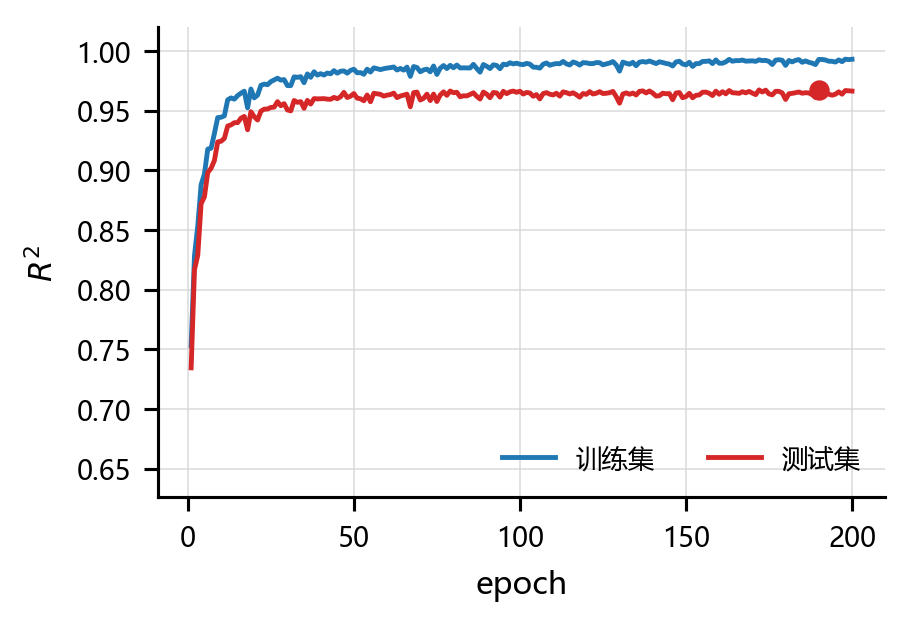
\includegraphics[width=\columnwidth]{net_train_dnn_r2_zh.png}\\[-0.2em]
{\scriptsize (a) 全量 DNN}\\[0.45em]
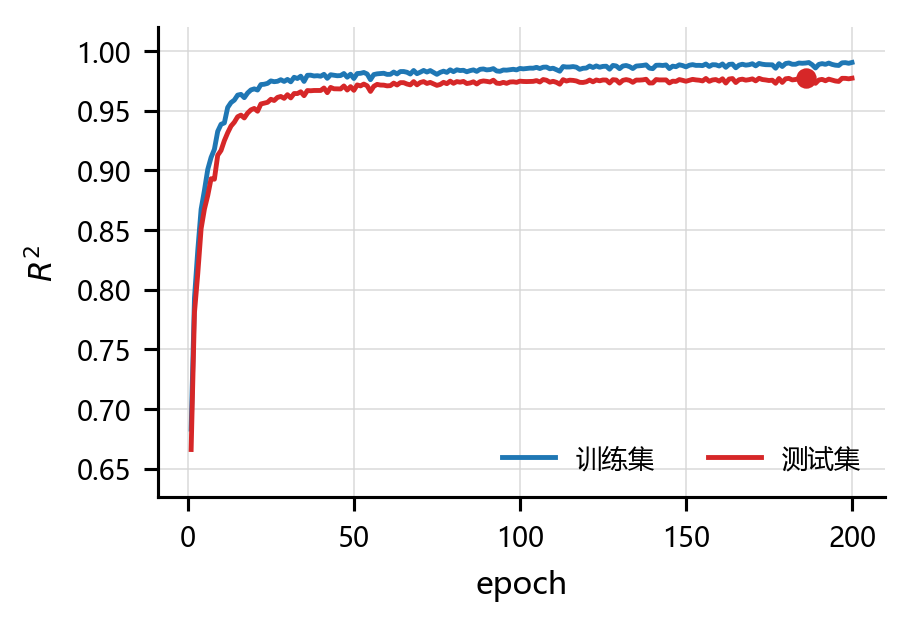
\includegraphics[width=\columnwidth]{net_train_l1_r2_zh.png}\\[-0.2em]
{\scriptsize (b) L1GateDNN}
\figbicaption{净实际交换功率目标上统一刻度的 $R^2$ 训练过程对比}{Training $R^2$ processes with unified scales for net actual interchange}
\label{fig:train_pair}
\end{figure}

图~\ref{fig:l1_gate} 展示了 L1GateDNN 的门控参数演化。每条曲线对应一个候选字段的 gate 值。训练初期，不同字段门控值出现明显分化；随着 L1 惩罚持续作用，大量弱贡献字段逐步衰减到阈值以下，少量关键字段维持较高 gate 值。最终阈值 0.10 下保留 18 个字段，其中包含 \code{gen\_fuel\_gas\_mw}、\code{gen\_fuel\_coal\_mw}、\code{total\_pjm\_rt\_load\_mwh}、\code{metered\_load\_mw}、\code{prelim\_load\_avg\_hourly} 和 \code{gen\_fuel\_solar\_mw} 等。图~\ref{fig:l1_active} 则显示活跃字段数量逐渐下降并趋于稳定，说明模型不是在训练末尾一次性截断，而是在优化过程中逐步形成紧凑推断源集合。

\begin{figure}[H]
\centering

\includegraphics[width=\columnwidth]{net_l1_gate_params_zh.png}
\figbicaption{净实际交换功率目标上门控参数 gate 的演化}{Gate values over epochs for net actual interchange}
\label{fig:l1_gate}
\end{figure}

\begin{figure}[H]
\centering

\includegraphics[width=\columnwidth]{net_l1_active_features_zh.png}
\figbicaption{净实际交换功率目标上活跃字段数量的演化}{Number of active features over epochs}
\label{fig:l1_active}
\end{figure}

\subsection{Top-n 推断源验证}
为验证 L1GateDNN 所选字段是否具有实际推断能力，按照最终 gate 值排序，分别取 Top3、Top6、Top9、Top12、Top15、Top18 字段训练普通 DNN，并与全量 55 字段和未选中 37 字段进行比较。图~\ref{fig:top_series} 给出结果。Top3 和 Top6 由于字段数过少，$R^2$ 分别仅为 0.4469 和 0.5778；当字段数增加到 Top9 时，$R^2$ 提升至 0.9186；Top15 达到 0.9630；Top18 达到 0.9681，略高于全量 55 字段的 0.9661。相反，去除 Top18 后剩余 37 字段单独训练仅取得 0.7820。这说明 L1 门控并非简单挑选单个强相关字段，而是识别出能够共同支撑目标推断的核心字段集合；未选中字段虽然数量更多，但缺少关键路径，推断能力明显下降。

\begin{figure}[H]
\centering

\includegraphics[width=\columnwidth]{net_top_series_r2_zh.png}
\figbicaption{净实际交换功率目标上的 Top-n 推断源验证}{Top-n inference-source validation}
\label{fig:top_series}
\end{figure}

\subsection{改进门控边界学习}
图~\ref{fig:improved_gate} 至图~\ref{fig:improved_b} 展示了相关性驱动改进门控的训练结果。与普通 L1 gate 不同，改进门控的 gate 由六维相关性向量经 Sigmoid 映射生成，因此图~\ref{fig:improved_gate} 中的分界阈值为 0.5，而不是普通 L1GateDNN 的 0.10。该设置具有明确数学含义：当 $W^{\mathrm{T}}R_i+b=0$ 时，Sigmoid 输出为 0.5，对应风险边界；高于 0.5 表示相关性证据足以使 gate 打开，低于 0.5 则表示字段更可能被压制。

在本次实验中，改进 L1 门控最终保留 17 个字段，best test $R^2=0.9726$。从权重演化看，HSIC 对应权重在训练后保持最高，说明非线性依赖证据对净实际交换功率目标的风险判断贡献较大；偏置 $b$ 从接近 0 逐步下降到约 -0.70，表明模型在 L1 压力下不断收紧 gate 打开条件。这一实验的意义在于，它把“六类相关性指标如何共同决定字段风险”转化为可学习边界，而不是依赖人工给每个指标设置孤立阈值。

\begin{figure}[H]
\centering

\includegraphics[width=\columnwidth]{improved_l1_gate_params_zh.png}
\figbicaption{改进 L1 门控的 gate 值演化}{Gate evolution of the improved L1 gate}
\label{fig:improved_gate}
\end{figure}

\begin{figure}[H]
\centering
\begin{minipage}{\columnwidth}
\centering
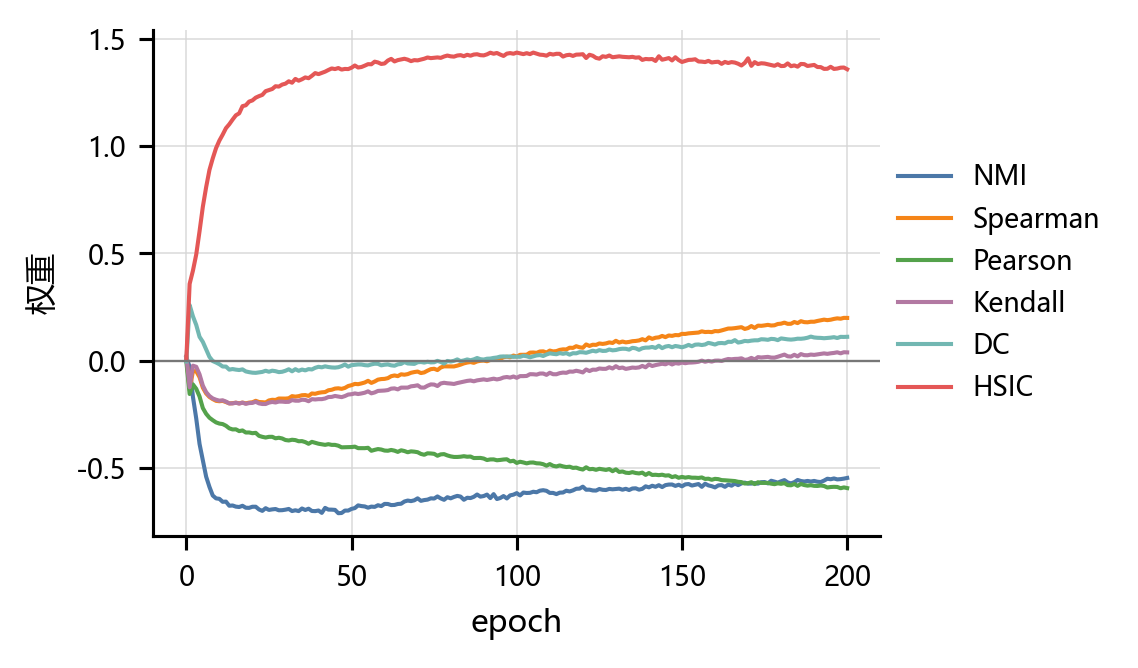
\includegraphics[width=0.92\linewidth]{improved_l1_w_meta_zh.png}\\[-0.4em]
{\scriptsize (a) 相关性指标权重 $W$}
\end{minipage}\\[-0.2em]
\begin{minipage}{\columnwidth}
\centering

\includegraphics[width=0.86\linewidth]{improved_l1_b_meta_zh.png}\\[-0.4em]
{\scriptsize (b) 偏置 $b$}
\end{minipage}
\figbicaption{改进门控中的指标权重与偏置演化}{Evolution of metric weights and bias}
\label{fig:improved_b}
\end{figure}

\section{多目标对比实验}
\subsection{DNN 与 L1DNN 直接对比}
为了先展示本文方法本身的效果，本文在 12 个敏感目标上比较全量 DNN 与 L1DNN 选中特征 DNN。这里“全量 DNN”表示在当前目标允许的全部字段上训练，不考虑 L1 门控系统的筛选；“L1DNN 选中特征”表示先由 L1GateDNN 得到活跃字段，再使用相同 DNN 结构重新训练评估。结果见图~\ref{fig:dnn_l1_compare} 和表~\ref{tab:dnn_l1_compare}。

从平均结果看，若按数据全集中 70 个数值字段扣除目标字段后的 69 个字段作为统一全量口径，则全量 DNN 字段利用率为 100\%，平均 $R^2$ 为 0.9031；L1DNN 平均使用 15.50 个字段，字段利用率约为 22.46\%，平均 $R^2$ 为 0.9111。在 \code{congestion\_price\_da}、\code{da\_as\_total\_mw\_primary\_reserve}、\code{gross\_actual\_interchange\_mw}、\code{net\_actual\_interchange\_mw} 等目标上，L1DNN 明显或略微优于全量 DNN；在 \code{congestion\_price\_rt} 和 \code{total\_lmp\_da} 上，L1DNN 略低于全量 DNN。这说明所提方法不是对所有目标机械压缩，而是在大多数目标上能以较小字段集合保持同等甚至更强的泛化能力。

\begin{figure}[H]
\centering

\includegraphics[width=\columnwidth]{dnn_vs_l1_method_compare_zh.png}
\figbicaption{12 个敏感目标上的全量 DNN 与 L1DNN 对比}{Comparison between all-feature DNN and L1DNN}
\label{fig:dnn_l1_compare}
\end{figure}

\begin{table}[H]
\centering
\scriptsize
\setlength{\tabcolsep}{2pt}
\tabbicaption{全量 DNN 与 L1DNN 选中特征对比}{All-feature DNN and L1DNN-selected feature comparison}
\label{tab:dnn_l1_compare}
\begin{tabularx}{\columnwidth}{Xrrrr}
\toprule
中心目标 & 全量字段 & L1 字段 & 全量 DNN & L1DNN \\
\midrule
拥塞价 DA & 69 & 2 & 0.9408 & \textbf{0.9954} \\
主备用容量 & 67 & 14 & 0.8495 & \textbf{0.8826} \\
总实际交换 & 69 & 16 & 0.8499 & \textbf{0.8677} \\
30 min 备用容量 & 68 & 22 & 0.8967 & \textbf{0.9086} \\
边际损耗价 DA & 69 & 18 & 0.8936 & 0.8995 \\
净实际交换 & 67 & 18 & 0.9680 & 0.9728 \\
总发电量 & 42 & 16 & 0.9253 & 0.9271 \\
净计划交换 & 67 & 16 & 0.9691 & 0.9694 \\
总损耗 & 69 & 18 & 0.9413 & 0.9409 \\
计量负荷 & 42 & 15 & 0.9157 & 0.9139 \\
日前 LMP & 66 & 13 & \textbf{0.9622} & 0.9510 \\
拥塞价 RT & 69 & 18 & \textbf{0.7255} & 0.7040 \\
\midrule
平均 & -- & 15.5 & 0.9031 & 0.9111 \\
\bottomrule
\end{tabularx}
\end{table}

\subsection{同预算 baseline 对比}
为了回应“baseline 的字段数 $n$ 是否由 L1DNN 单方面决定”的公平性问题，本文进一步采用同预算策略。具体做法是：先用 L1GateDNN 在特征预算序列上搜索，当某个 $n$ 使 L1GateDNN 的 $R^2$ 达到全量 DNN 的 95\% 或 97\% 时，锁定该 $n$；若继续增加若干候选预算仍无法达到目标，则采用当前可获得的最佳 $n$。随后所有 baseline 方法在相同 $n$ 下选择字段，并统一使用普通 DNN 训练测试。这样，比较对象不再是“谁选择更多字段”，而是在同一字段预算下“谁选择的字段更有推断能力”。

图~\ref{fig:budget_lines} 给出 95\% 与 97\% 统一预算下各目标的测试 $R^2$ 折线对比，图~\ref{fig:budget_avg} 进一步汇总平均结果。95\% 预算下，平均字段数为 8.92，L1GateDNN 平均 $R^2$ 为 0.8875，高于 RandomForest 的 0.8562、ElasticNet 的 0.8115、Lasso 的 0.7967 和 XGBoost 的 0.7798；97\% 预算下，平均字段数增加到 9.75，L1GateDNN 平均 $R^2$ 提升到 0.8943，仍优于各 baseline。两种预算下，单相关性方法整体偏低，说明仅依靠 NMI、Pearson 或 Spearman 排序难以稳定保留联合推断路径；树模型和线性稀疏模型虽在部分目标上表现较好，但平均上仍低于 L1GateDNN。

\begin{figure}[H]
\centering

\includegraphics[width=\columnwidth]{budget95_baseline_lines_zh.png}\\[-0.2em]
{\scriptsize (a) 95\% 统一预算}\\[0.45em]

\includegraphics[width=\columnwidth]{budget97_baseline_lines_zh.png}\\[-0.2em]
{\scriptsize (b) 97\% 统一预算}
\figbicaption{统一预算下不同目标的 baseline 测试 $R^2$ 折线对比}{Target-level baseline comparison under unified feature budgets}
\label{fig:budget_lines}
\end{figure}

\begin{figure}[H]
\centering

\includegraphics[width=\columnwidth]{budget95_average_bar_zh.png}\\[-0.2em]
{\scriptsize (a) 95\% 统一预算}\\[0.45em]

\includegraphics[width=\columnwidth]{budget97_average_bar_zh.png}\\[-0.2em]
{\scriptsize (b) 97\% 统一预算}
\figbicaption{统一预算下不同 baseline 的平均测试 $R^2$}{Average baseline comparison under unified feature budgets}
\label{fig:budget_avg}
\end{figure}

\section{冗余噪声影响分析}
\subsection{训练曲线对比}
在部分目标上，少量 L1 选中特征的测试 $R^2$ 高于全量字段 DNN。该现象并不意味着全量字段信息不足，而是说明全量输入中存在冗余和噪声字段，普通 MLP 在有限样本下可能受到干扰，出现训练集拟合持续提高而测试集泛化下降的过拟合现象。为验证这一解释，本文选择差异更明显的 \code{congestion\_price\_da} 和 \code{da\_as\_total\_mw\_primary\_reserve} 两个目标，比较全量 DNN、L1GateDNN 和 L1 选中特征再训练 DNN 的训练曲线。

图~\ref{fig:redundant_curve} 与表~\ref{tab:noise_curve} 显示，\code{congestion\_price\_da} 上全量 DNN 的 best test $R^2$ 为 0.9408，最终训练/测试泛化差距约 0.0621；而仅使用 L1 选出的 2 个字段重新训练，best test $R^2$ 达到 0.9954，最终泛化差距仅 0.0025。\code{da\_as\_total\_mw\_primary\_reserve} 上，全量 DNN 的泛化差距约 0.1439，L1 选中特征 DNN 的 test $R^2$ 从 0.8495 提升到 0.8580。可见，字段压缩降低了模型对弱相关和噪声字段的记忆压力，使测试集表现更稳定。

\begin{figure}[H]
\centering
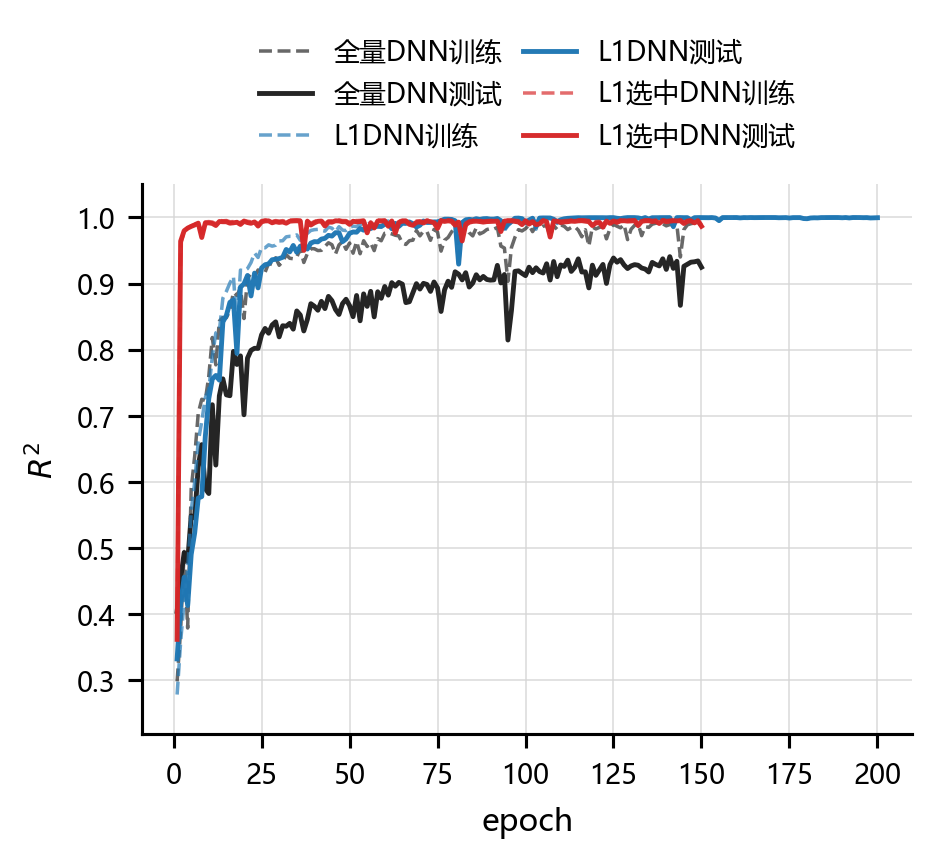
\includegraphics[width=\columnwidth]{redundant_training_congestion_zh.png}\\[-0.2em]
{\scriptsize (a) 阻塞价 DA}\\[0.45em]
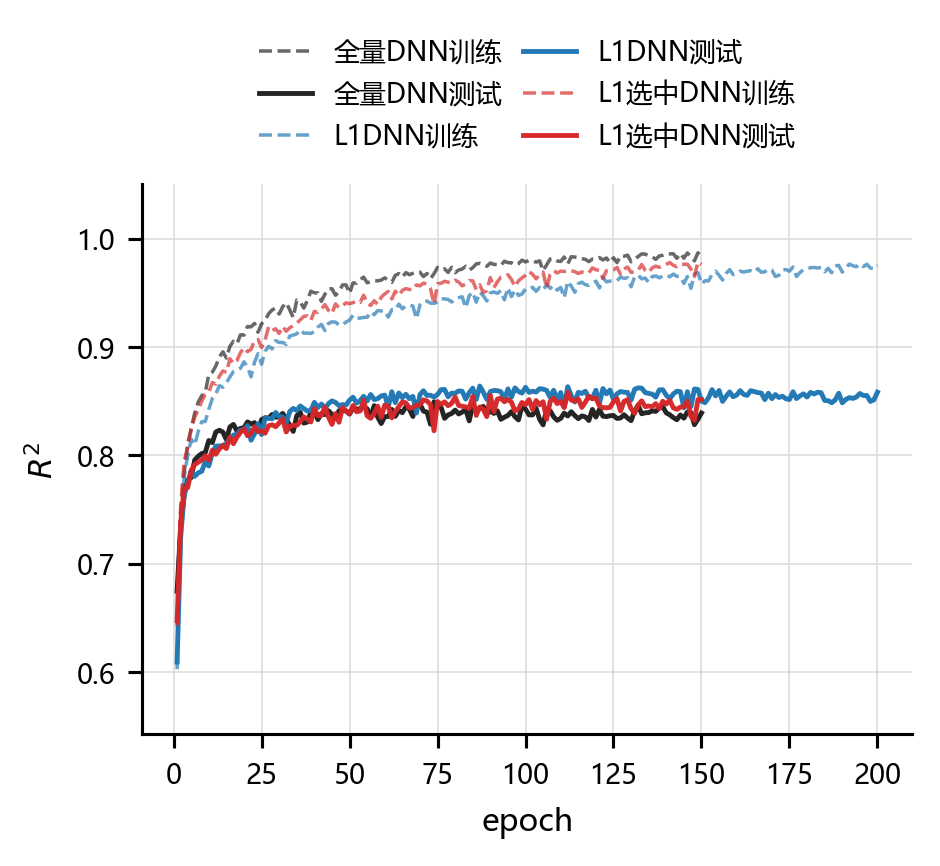
\includegraphics[width=\columnwidth]{redundant_training_primary_zh.png}\\[-0.2em]
{\scriptsize (b) 主备用容量}
\figbicaption{全量字段与 L1 选中特征的训练/测试 $R^2$ 曲线对比}{Train and test curves of all features and L1-selected features}
\label{fig:redundant_curve}
\end{figure}

\begin{table}[H]
\centering
\scriptsize
\setlength{\tabcolsep}{3pt}
\tabbicaption{冗余噪声解释实验的训练曲线统计}{Training-curve statistics for redundant-noise explanation}
\label{tab:noise_curve}
\textbf{(a) 拥塞价 DA}\\[-0.2em]
\begin{tabularx}{\columnwidth}{Xrrrr}
\toprule
方法 & 字段数 & Best $R^2$ & epoch & 泛化差距 \\
\midrule
全量 DNN & 69 & 0.9408 & 141 & 0.0621 \\
L1GateDNN & 69 & 1.0000 & 194 & -0.0001 \\
L1 选中特征 DNN & 2 & 0.9954 & 139 & 0.0025 \\
\bottomrule
\end{tabularx}

\vspace{0.4em}
\textbf{(b) 主备用容量}\\[-0.2em]
\begin{tabularx}{\columnwidth}{Xrrrr}
\toprule
方法 & 字段数 & Best $R^2$ & epoch & 泛化差距 \\
\midrule
全量 DNN & 67 & 0.8495 & 74 & 0.1439 \\
L1GateDNN & 67 & 0.8639 & 87 & 0.1170 \\
L1 选中特征 DNN & 35 & 0.8580 & 112 & 0.1247 \\
\bottomrule
\end{tabularx}
\end{table}

\subsection{Top-n 递增实验}
进一步地，本文按照 L1 gate 排名逐渐增加字段数，观察测试 $R^2$ 的变化。图~\ref{fig:topn_noise} 给出两个目标的完整 Top-n 序列，并用三角形标出最高点。\code{congestion\_price\_da} 在 Top2 时已经达到 0.9954，Top3 提升到 0.9999，继续增加到 Top24 仍保持高水平，但 Top32 下降到 0.9851；全量 69 字段仅为 0.9408。对于 \code{da\_as\_total\_mw\_primary\_reserve}，$R^2$ 随字段数从 Top1 到 Top24 逐步提升至 0.8872，但继续增加到 Top32 和 Top35 后下降到 0.8545 和 0.8536，接近全量 DNN 的 0.8495。该结果说明，关键字段数量不足时模型无法恢复目标；字段数量达到合理区间后推断能力显著提高；当继续加入弱贡献字段时，冗余噪声会增加模型复杂度，导致泛化收益下降甚至反向。

\begin{figure}[H]
\centering

\includegraphics[width=\columnwidth]{topn_congestion_zh.png}\\[-0.2em]
{\scriptsize (a) 阻塞价 DA}\\[0.45em]

\includegraphics[width=\columnwidth]{topn_primary_zh.png}\\[-0.2em]
{\scriptsize (b) 主备用容量}
\figbicaption{按 L1 gate 排名逐步增加字段数的测试 $R^2$、最高点及全量点}{Test $R^2$ with incrementally added Top-n features, peak markers and full-feature points}
\label{fig:topn_noise}
\end{figure}

\section{讨论}
实验结果表明，L1GateDNN 的优势并不只是平均 $R^2$ 略高，而在于其输出形式更适合数据发布审查。全量 DNN 可以证明目标可被预测，却无法定位推断路径；单相关性方法可以说明字段两两相关，却无法判断联合推断中的不可替代性；线性稀疏模型和树模型能够给出排序，但其排序未必与 DNN 推断能力一致。L1GateDNN 将门控选择嵌入非线性推断训练过程，使字段是否保留直接受到预测误差和稀疏约束共同约束，因此更接近“哪些字段会被攻击模型实际利用”的风险语义。

同预算 baseline 进一步说明，固定字段数 $n$ 并不是为了偏向 L1DNN，而是为了构造可解释的特征预算。若让每种方法任意选择不同数量字段，则性能差异可能来自字段数差异而非选择质量。本文采用 95\% 和 97\% 两组预算，一方面展示低容忍度下 L1GateDNN 的领先优势，另一方面展示更高容忍度下各方法接近全量 DNN 的趋势。对于个别目标，如果达到 97\% 需要明显增加字段数或若干预算点提升不明显，则采用最佳可用预算，以避免为了追求阈值而引入过多冗余字段。

少量字段优于全量字段的现象也具有实际含义。在电力数据表中，很多字段并非独立信息源，而是由同一物理过程或市场机制派生出来。全量输入会把这些共线、弱相关或噪声字段同时交给 MLP，增加模型记忆训练样本细节的机会。L1 门控先筛出稳定推断路径，再进行普通 DNN 验证，相当于降低了输入维度和过拟合风险。因此，字段压缩并不是牺牲信息，而是在保留核心信息的同时减少噪声干扰。

本文仍存在一些局限。第一，L1 正则强度和活跃阈值会影响最终字段数量，实际应用中需要根据发布场景设置风险严格程度。第二，部分敏感目标可能存在多个等价推断路径，单次训练得到的字段集合不一定唯一，后续应增加多随机种子和多时间窗口稳定性分析。第三，本文主要以单目标为中心识别风险源，多目标之间的联合泄露和风险传播仍需进一步建模。

\section{结论}
本文围绕电力数据共享中的隐含推断风险问题，提出了多相关性筛选与 L1 门控深度神经网络相结合的分析方法。该方法先通过六类相关性指标保留潜在候选字段，再利用 L1GateDNN 在保持敏感目标推断能力的同时压缩冗余字段，并通过普通 DNN 再训练验证所选字段集合的实际推断能力。相关性驱动的改进门控进一步把多相关性证据映射为统一风险边界，增强了方法的解释性。

基于 PJM 2025 年小时级数据的实验表明，针对净实际交换功率目标，所提方法从 55 个候选字段中筛选出 18 个活跃字段，Top18 普通 DNN 验证 $R^2$ 为 0.9681，高于全量字段结果 0.9661，而未选中字段单独推断仅为 0.7820。在 12 个敏感目标上，L1DNN 以平均 15.5 个字段取得 0.9111 的平均测试 $R^2$，高于全量 DNN 的 0.9031；95\% 和 97\% 同预算 baseline 中，L1GateDNN 也保持最高平均 $R^2$。冗余噪声解释实验进一步说明，全量输入中的弱相关和冗余字段会增加过拟合风险，合理特征压缩有助于提升泛化性能。上述结果说明，所提方法可为电力数据发布前的字段审查、敏感等级调整和隐含推断路径阻断提供参考。

未来工作将从三个方向展开：一是引入多随机种子和跨月份时间窗口，评估门控字段集合的稳定性；二是将单目标推断扩展为多目标风险图谱，描述不同敏感字段之间的联合泄露关系；三是把识别出的风险源集合与字段降精度、延迟发布、分级授权等处置策略结合，形成面向实际数据共享流程的闭环防护机制。

\balance
\begin{thebibliography}{99}
\bibitem{ref-liu-cps}
Liu T, Tian J, Wang J, et al. Integrated security threats and defense of cyber-physical systems[J]. Acta Automatica Sinica, 2019, 45(1): 5-24.

\bibitem{ref-ma-pjm}
Ma Z, Zhang H, Zhu L. Information disclosure system in American electricity market and its enlightenment for China[J]. Automation of Electric Power Systems, 2017, 41(24): 49-57.

\bibitem{ref-fan-pjm}
Fan Z, Horger T, Bastian J, et al. An overview of PJM energy market design and development[C]//2008 Third International Conference on Electric Utility Deregulation and Restructuring and Power Technologies. Piscataway: IEEE, 2008: 12-17.

\bibitem{ref-sankar}
Sankar L, Rajagopalan S R, Mohajer S, Poor H V. Smart meter privacy: A theoretical framework[J]. IEEE Transactions on Smart Grid, 2013, 4(2): 837-846.

\bibitem{ref-giaconi}
Giaconi G, Gündüz D, Poor H V. Privacy-aware smart metering: Progress and challenges[J]. IEEE Signal Processing Magazine, 2018, 35(6): 59-78.

\bibitem{ref-adewole}
Adewole K S, Torra V. Privacy issues in smart grid data: from energy disaggregation to disclosure risk[C]//International Conference on Database and Expert Systems Applications. Cham: Springer, 2022: 71-84.

\bibitem{ref-lan-load}
Lan D, Zhu H, Wu J, et al. A short-term load forecasting method of distribution network based on improved AlexNet-GRU deep learning network[C]//2021 IEEE 5th Conference on Energy Internet and Energy System Integration. Piscataway: IEEE, 2021: 3004-3010.

\bibitem{ref-jiao-pv}
Jiao X, Sun Y, Peng D, et al. Photovoltaic power abnormal data cleaning based on variance change point and correlation analysis[C]//2021 6th International Conference on Power and Renewable Energy. Piscataway: IEEE, 2021: 1140-1145.

\bibitem{ref-deng-load}
Deng X, Zhang C, Peng H, et al. Short-term load forecasting for regional power grids based on correlation analysis and feature extraction[C]//2022 7th Asia Conference on Power and Electrical Engineering. Piscataway: IEEE, 2022: 1081-1085.

\bibitem{ref-szekely-dcorr}
Székely G J, Rizzo M L, Bakirov N K. Measuring and testing dependence by correlation of distances[J]. The Annals of Statistics, 2007, 35(6): 2769-2794.

\bibitem{ref-gretton-hsic}
Gretton A, Bousquet O, Smola A, Schölkopf B. Measuring statistical dependence with Hilbert-Schmidt norms[C]//Algorithmic Learning Theory. Berlin: Springer, 2005: 63-77.

\bibitem{ref-wang-meter}
Wang Y, Chen Q, Hong T, Kang C. Review of smart meter data analytics: Applications, methodologies, and challenges[J]. IEEE Transactions on Smart Grid, 2019, 10(3): 3125-3148.

\bibitem{ref-breiman-rf}
Breiman L. Random forests[J]. Machine Learning, 2001, 45(1): 5-32.

\bibitem{ref-chen-xgboost}
Chen T, Guestrin C. XGBoost: A scalable tree boosting system[C]//Proceedings of the 22nd ACM SIGKDD International Conference on Knowledge Discovery and Data Mining. New York: ACM, 2016: 785-794.

\bibitem{ref-tibshirani-lasso}
Tibshirani R. Regression shrinkage and selection via the lasso[J]. Journal of the Royal Statistical Society: Series B, 1996, 58(1): 267-288.

\bibitem{ref-zou-enet}
Zou H, Hastie T. Regularization and variable selection via the elastic net[J]. Journal of the Royal Statistical Society: Series B, 2005, 67(2): 301-320.

\bibitem{ref-xing-micdnn}
Xing Z, Wang Z, Feng J, et al. MIC-DNN: Data-driven correlation analysis framework for power data[C]//2025 40th Youth Academic Annual Conference of Chinese Association of Automation. Piscataway: IEEE, 2025: 2969-2974.
\end{thebibliography}

\section*{收稿日期与作者简介}
\noindent\textbf{收稿日期：}20XX-XX-XX

\noindent\textbf{作者简介：}\par
\noindent 杜浩存（出生年），男，研究方向为电力数据安全、信息物理系统安全与机器学习安全，邮箱：待补充。

\end{multicols}

\end{document}

